\section{Introduction} \label{sec:intro}



We consider problems where a decisionmaker faces $n$ alternatives.
Each alternative represents a potential reward, but involves search costs and decisions under uncertainty to discover such a reward.
The decisionmaker may adaptively interact with the alternative search processes over time, but must eventually select only one alternative's reward (more generally, a feasible subset of rewards).

A special case is the \emph{Pandora's Box} model, originally developed by \citet{weitzman1979optimal}, where the alternatives are imagined as ``boxes'' that may be ``opened'' at a cost to reveal the reward inside.
An application (e.g. \citet{kleinberg2016descending}) is when a valuable asset such as a house or startup is for sale, and each potential buyer must invest in inspection or due diligence to learn their value; only one can get the house.
This model is well-studied, including extensions such as ``non-obligatory'' inspection~\citep[e.g.]{doval2018whether,beyhaghi2019pandora}, multiple stages of inspection~\citep[e.g.]{kleinberg2016descending,bowers2024matching}, and combinatorial constraints~\citep{singla2018price,gupta2019markovian} (see Section \ref{subsec:related}).

We consider generalizations where each box is replaced by a \emph{Markov Search Process (MSP)}, which involves a finite sequence of costly decisions and stochastic state transitions culminating in an available reward.
As another motivating example, suppose a company is involved in research and development on several potential new products, but only has the capacity to bring one to market.
Each product development is a Markov Search Process involving choices between a number of means -- experiments, prototype development, and so on -- to further develop it; each choice requires an investment of resources and may open the door to further choices or investments depending on the outcomes of prior stages.
The company may interactively investigate and develop the potential products in parallel, e.g. abandoning some when they become less promising and perhaps revisiting them later; but eventually, it must choose only one product to produce.

As we discuss below, prior work on such problems tends to either rely on index theorems related to Weitzman's; or where index theorems are unavailable, focus on details of a particular model, e.g. non-obligatory Pandora's Box.
Techniques for provable guarantees in more broad decisionmaking settings are generally unavailable.
It might therefore be expected for our problem that, even in the case of selecting a single reward, an efficient approximation is either not possible, or requires a highly adaptive approach.

Neither turns out to be the case.
In this paper, we give polynomial-time constant-factor approximation algorithms for this problem and for the extension to the case of any matroid selection constraint.
Our algorithms are online, i.e. process the alternatives one at a time, yielding optimal prophet inequalities for this setting.
Our results also imply a constant Price of Anarchy for the problem of coordinating an arbitrary group of strategic agents, each of whom faces a costly investment environment modeled as an MSP, to efficiently search for potential uses of constrained resource(s) and allocate them.

\subsection{Main result} \label{subsec:intro-main}

\subsubsection{Problem setting}
A \emph{Markov Search Process (MSP)} $\M$ is a variant of a Markov Decision Process.
Beginning with a start state, a decisionmaker may select between multiple costly actions, each resulting in a stochastic transition to a new state.
Eventually, the process reaches a halting state and an available reward is revealed.
Unlike in a Markov decision process, there is no discounting, actions only incur costs (not rewards) and the state transitions form a directed acyclic graph (DAG).

In our main problem, \emph{Combinatorial Markov Search}, a decisionmaker faces $n$ available MSPs $\M_1,\dots,\M_n$ and may interact with them adaptively, incurring costs and eventually revealing at most one available reward per process.
The decisionmaker must, in the end, select only one of the corresponding discovered rewards, or more generally, some feasible subset of $[n] := \{1,\dots,n\}$ subject to e.g. a matroid or other downward-closed constraint.
The objective is to maximize \emph{welfare}, the sum of the selected rewards minus the sum of all incurred search costs.
The problem is related to \emph{superprocesses}~\citep{nash1973optimal}, which are similar in spirit but generally involve Markov Decision Processes and time discounting (see Section \ref{subsec:related}).

Even very special cases of this problem are challenging.
For example, the NP-hard problem of Pandora's Box with nonobligatory inspection~\citep{fu2023pandora,beyhaghi2023pandora} is the case where each MSP is a ``box'' representing a single decision (to open or not open the box), the reward structures of the decisions are closely linked (an expected reward for a closed box versus an inspection cost and available reward for an open box), and the constraint is a ``rank one matroid'', i.e. only one of the $n$ rewards can be taken.

\subsubsection{Going beyond index theorems}

A main challenge is that the problem appears to be highly interactive.
When do we switch from interacting with one process to another, and to which process?
In e.g. the special case of Pandora's Box vith multiple stages, or the related model of Multi-Armed Bandits, the solution is provided by index theorems (\citet{weitzman1979optimal} and \citet{gittins1979bandit} respectively).
An index theorem provides a locally-computable index that depends only on a given alternative (a nested Pandora box, a one-armed bandit) and that determines the globally optimal policy.
Almost all approaches to superprocesses and similar problems of which we are aware involve finding sufficient conditions for an index theorem to hold; examples include \citet{whittle1980multi,glazebrook1982sufficient,keller2003branching,gupta2019markovian}, and others discussed in Section \ref{subsec:related}.
Such theorems have powered a number of results in mechanism design~\citep{kleinberg2016descending,bowers2023high, immorlica2020information} and combinatorial optimization~\citep{singla2018price,gupta2019markovian}.
But we do not know of any robust approximations for such settings that extend broadly beyond where index theorems hold.
We ask: \textbf{Are there robust, approximate, and local index-like strategies for highly interactive search processes?}

We show that a very natural local-to-global technique answers in the positive.
In fact, we can use this technique to interact with the alternatives $i=1,\dots,n$ one at a time, online.
When MSP $i$ arrives, the algorithm will interact with it, make an irrevocable take-it-or-leave it decision, and move on to $i+1$.
An approximation guarantee by such an algorithm, relative to the offline adaptive optimal, is known as a \emph{prophet inequality}.
\begin{theorem*}[Main result, Corollary \ref{cor:dags-matroid-approx}]
  For the problem of Combinatorial Markov Search subject to any matroid feasibility constraint, there exists an online algorithm running in time polynomial in the input size and $\frac{1}{\epsilon}$ that, given any $\epsilon > 0$, guarantees a prophet inequality of $\frac{1}{2} - \epsilon$.
\end{theorem*}
Of course, a $\frac{1}{2}$ factor is known to be tight for online algorithms even in the case where a single reward must be chosen from a list of independent random values~\citep{samuelcahn1984comparison}.


\subsubsection{The single-agent utility problem}

In online selection tasks such as prophet inequalities, algorithms typically select arriving values only if they exceed a given threshold.
Thresholds correspond to posted-price mechanisms: an arriving agent maximizes utility by buying if and only if their value exceeds their price.
Our local-to-global idea is to extend posted pricing to the setting where agents, faced with a posted price, conduct their search problem optimally under the assumption that, when they eventually reveal a prize, they will need to pay the posted price in order to actually claim it.
We call this the \emph{single-agent utility problem (\SAUP{})}.
\begin{prop*}[Proposition \ref{prop:max-saup}]
  For a given Markov Search Process $\M$ and threshold $\tau$, the single-agent utility problem \SAUP{}$(\M,\tau)$ can be solved in polynomial time.
\end{prop*}
To design and analyze this algorithm, we make heavy use of Weitzman index theorem machinery, originally developed for the simpler ``nested'' or ``multi-stage'' Pandora's box problem, described below; along with a reduction to the ``Pandora's Cabinets'' model that we also introduce below.

Our matroid prophet algorithm in particular uses \SAUP{} to interact with each arrival. Accordingly, we refer to it as \emph{\SAUP-based}.
An implication is the existence of mechanisms with a Price of Anarchy (i.e. welfare approximation) of $\frac{1}{2}$ for serving single-parameter agents, who conduct search processes to discover their values for service, subject to a matroid constraint.
However, the analysis is not as simple as combining our efficient \SAUP{} algorithm with a known prophet inequality; we will need to build the result through a series of reductions.


\subsection{Techniques: bandits, cabinets, and DAGS}

\begin{figure}
	\centering
	\begin{subfigure}[b]{0.2\textwidth}
		\centering
		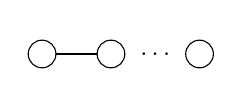
\begin{tikzpicture}[
			wide/.style={line width=4pt}, every node/.style={circle,draw,minimum size=10}, scale=.25]

			\node (root) at (-3.5,0) {};
			\node (child) at (0,0) {};
			\node (end) at (4.5,0) {};

			\draw (root) -- (child);
			\path (child) -- (end) node[midway, draw=none,fill=none] {\small $\dots$};

		\end{tikzpicture}
		\subcaption{}\label{subfig:multistage-pandora}
	\end{subfigure}
	\hfil
	\begin{subfigure}[b]{0.2\textwidth}
		\centering
		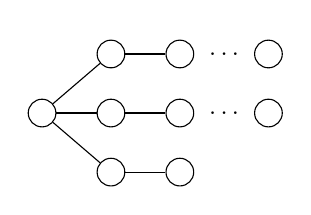
\begin{tikzpicture}[
			wide/.style={line width=4pt}, every node/.style={circle,draw,minimum size=10}, scale=.25]

			\node (root) at (-7, 0) {};

			\node (s1) at (-3.5,3) {};
			\node (s2) at (0,3) {};
			\node (s3) at (4.5,3) {};

			\draw (s1) -- (s2);
			\path (s2) -- (s3) node[midway, draw=none,fill=none] {\small $\dots$};

			\node (s4) at (-3.5,0) {};
			\node (s5) at (0,0) {};
			\node (s6) at (4.5,0) {};

			\draw (s4) -- (s5);
			\path (s5) -- (s6) node[midway, draw=none,fill=none] {\small $\dots$};

			\node (s7) at (-3.5,-3) {};
			\node (s8) at (0,-3) {};

			\draw (s7) -- (s8);

			\draw (root) -- (s1);
			\draw (root) -- (s4);
			\draw (root) -- (s7);
		\end{tikzpicture}
		\subcaption{}\label{subfig:cabinets}
	\end{subfigure}
	\hfil
	\begin{subfigure}[b]{0.2\textwidth}
		\centering
		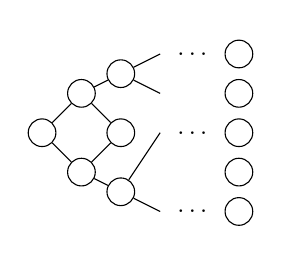
\begin{tikzpicture}[
			wide/.style={line width=4pt}, every node/.style={circle,draw,minimum size=10}, scale=.25]

			\node (root) at (-4,0) {};

			\node (s1) at (-2, 2) {};
			\node (s2) at (-2, -2) {};

			\node  (s3) at (0, 3) {};
			\node  (s4) at (0, 0) {};
			\node  (s5) at (0, -3) {};

			\coordinate  (s6) at (2, 4) {};
			\coordinate  (s7) at (2, 2) {};
			\coordinate  (s8) at (2, 0) {};
			\coordinate  (s9) at (2,-4) {};

			\node (b1) at (6, 4) {};
			\node (b2) at (6, 2) {};
			\node (b3) at (6, 0) {};
			\node (b4) at (6, -2) {};
			\node (b5) at (6, -4) {};

			\draw (root) -- (s1);
			\draw (root) -- (s2);

			\draw (s1) -- (s3);
			\draw  (s1) -- (s4);

			\draw  (s2) -- (s4);
			\draw  (s2) -- (s5);

			\draw (s3) -- (s6);
			\draw (s3) -- (s7);

			\draw (s5) -- (s8);
			\draw (s5) -- (s9);

			\path (s6) -- (b1) node[midway, draw=none,fill=none] {\small $\dots$};
			\path (s8) -- (b3) node[midway, draw=none,fill=none] {\small $\dots$};
			\path (s9) -- (b5) node[midway, draw=none,fill=none] {\small $\dots$};
		\end{tikzpicture}
		\subcaption{}\label{subfig:pandora-full-tree}
	\end{subfigure}
	\caption{\textbf{Bandits, Cabinets, and DAGs.}
		Simplified view of several decisionmaking structures considered in this paper.
		Time moves from left to right.
        Edges from each state node show possible actions, where the out degree is the number of available actions at a given state.
		Each decision incurs a cost and results in a stochastic state transition (omitted from the figure to focus on the differences in settings).
		(\ref{subfig:multistage-pandora}) represents a \emph{bandit process} where there is only one available action from every state, i.e. to advance the process.
		(\ref{subfig:cabinets}) represents \emph{Pandora's Cabinets} model in which there is an initial decision between several alternatives (i.e. which ``drawer'' to open), and each alternative is a bandit process.
		(\ref{subfig:pandora-full-tree}) represents the most general Markov Search Process model, where the state transitions may form an arbitrary DAG.
		In each of the settings in this paper, $n$ structures arrive sequentially, and each must be explored and either selected or discarded before the next comes.
	}
\end{figure}


To address Combinatorial Markov Search, we initially consider easier versions where each search process $i=1,\dots,n$ has a simpler structure.

\subsubsection{Bandits and Cabinets\dots}

The simplest case of our problem is a \textbf{bandit}: at each stage, one can either ``advance'' the bandit, incurring a cost and observing a stochastic transition; or halt.
Eventually, the bandit in our setting reaches a ``sink'' state at which a reward is revealed.
The offline problem (with a rank-one matroid constraint) is exactly Pandora's Box with Nested Boxes, also called Multi-Stage Pandora's Box~\citep{kleinberg2016descending,bowers2024matching}.
In this case, a generalized Weitzman index theorem is known (see Section \ref{subsec:related}); the problem has also been studied with combinatorial objectives and constraints~\citep{gupta2019markovian}.

Our first contribution (Section \ref{sec:non-pandora}) is the case where each search process $i=1,\dots,n$ is a modeled as a \textbf{cabinet}\footnote{We acknowledge Bobby Kleinberg for the imagery of this name for the problem.} containing $m_i$ drawers.
Each drawer $j$ contains a random reward $X_i^j$, but only one drawer per cabinet may ever be opened.
After opening one drawer $j(i)$ from each cabinet $i$, a subset $F \subseteq 2^{[n]}$ may be selected subject to the feasibility constraint, with total welfare $\sum_{i \in F} X_i^{j(i)}$.
This is therefore a type of stochastic probing~\citep{asadpour2016maximizing} problem, which in the online setting we call \emph{Cabinets-Prophets}.
We prove the following.

\begin{theorem*}[Theorem \ref{thm:classic-cp-dc}]
  Let $\F \subseteq 2^{[n]}$ be any downward-closed constraint system.
  If $\F$ has an ex-ante prophet inequality of $\alpha(n)$ for the classic prophets setting, then it has an ex-ante prophet inequality of $\alpha(n)$ for the Cabinets-Prophets problem.
\end{theorem*}
If the feasible polytope for $\F$ has an efficient separation oracle, we attain computational efficiency as well.
The use of the \emph{ex-ante} optimal (e.g. \citep{lee2018optimal}), which only must satisfy $\F$ in expectation, will be crucial for our main results later.
We note that the ex-ante optimal algorithm for Cabinets-Prophets is actually computable in polynomial time with convex optimization.
However, the reduction does not produce an \emph{incentive-compatible}, i.e. \SAUP{}-based algorithm.
In other words, unlike in classic prophet settings, incentive compatibility does not come for free.
We therefore manually provide the following.

\begin{theorem*}[Theorem \ref{thm:classic-cp-saup}]
  For the Cabinets-Prophets problem with any matroid constraint, there is a computationally efficient ``\SAUP{}-based'' ex-ante prophet inequality of $\frac{1}{2}$.
\end{theorem*}
For matroids, \citet{lee2018optimal} have given an ex-ante prophet inequality of $\frac{1}{2}$, but their algorithm does not immediately extend to a \SAUP{}-based algorithm for Cabinets-Prophets, as it is based on a Bernoulli instance reduction.
Instead, we show how to modify their proof to avoid the black-box Bernoulli reduction, then extend it to the Prophets-Cabinets setting in a \SAUP{}-compatible way.
We also add a nontrivial trick to allow $1-\epsilon$ approximations to the ex-ante optimal to give prophet inequalities with a $\frac{1-\epsilon}{2}$ guarantee, which will be useful later.


\subsubsection{\dots{}and Bandits in Cabinets\dots{}}

We next need one more intermediate setting.
In \emph{Pandora's Cabinets} problem (Section \ref{sec:cabinets}), we are given cabinets $i=1,\dots,n$ as before, but now each drawer $j$ contains a bandit process (i.e. a nested Pandora box).
An interactive $\OPT$ can open drawers and advance bandit processes at will.
But an online $\ALG$ must interact with each cabinet $i$ one at a time, selecting a drawer $j$ and either fully advancing or else discarding the observed bandit $\M_i^j$ before cabinet $i+1$ arrives.
As before, at most one drawer on a given cabinet can ever be opened.
For this problem, we are able to directly extend our results above.

\begin{theorem*}[Theorem \ref{thm:cp-pc}]
  Let $\F \subseteq 2^{[n]}$ be any downward-closed constraint system.
  If $\F$ has an ex-ante prophet inequality of $\alpha(n)$ for Cabinets-Prophets, then it has an ex-ante prophet inequality of $\alpha(n)$ for Pandora's Cabinets.
\end{theorem*}

\begin{figure}[h]
  \newcommand{\impliesthm}[1]{\parbox[c]{12ex}{\vskip2em \centering $\implies$ \\ {\centering \scriptsize Theorem \ref{#1}}}}
  \newcommand{\problemeff}[3]{\parbox[t]{#1}{\centering #2 \\ {\scriptsize (#3)}}}
  \newcommand{\problemeffone}[2]{\parbox[t]{#1}{\centering #2 \\ }}
  \label{fig:results-overview}

  {\small \hfill
  \addtolength{\tabcolsep}{-1.5ex}
  \begin{tabular}{ccccccc}
    \problemeffone{14ex}{Classic Prophets}
    &\impliesthm{thm:classic-cp-dc}
    &\problemeff{14ex}{Cabinets-Prophets}{cabinets}
    &\impliesthm{thm:cp-pc}
    &\problemeff{14ex}{Pandora's Cabinets}{bandits in cabinets}
    &\impliesthm{thm:pc-cms}
    &\problemeff{22ex}{Combinatorial Markov Search}{DAGs}
  \end{tabular}
  \hfill} 
  \caption{\textbf{Reductions.} Given any downward-closed constraint, an ex-ante prophet inequality for one setting implies one for the following setting.
    The approximation guarantee is preserved.
    However, computational efficiency and incentive compatibility are not necessarily preserved.
    In the case of matroid constraints, both efficiency and incentive compatibility can be preserved with a loss of an arbitrarily small $\epsilon$ in the approximation factor (Corollary \ref{cor:dags-matroid-approx}).
  } 
\end{figure}



\subsubsection{\dots{}and DAGs}

Our main and most general problem is \emph{Combinatorial Markov Search}: the decisionmaker faces $n$ available Markov Search Processes.
The heart of our solution is a reduction to Pandora's Cabinets problem.
The idea is straightforward: every deterministic policy $\pi$ on an MSP can be pictured as a drawer.
Inside the drawer is the bandit process defined by following the deterministic policy $\pi$ on the MSP: the only options are to continue with the deterministic policy, or else abandon the process.
Because it is a bandit, Weitzman index machinery can be applied.

Of course, this reduction naively results in a doubly-exponential blowup in the size of the problem (a policy is a function from the path traversed so far).
However, we show that Weitzman indices for bandits can be used, via backward induction, to efficiently construct an optimal deterministic policy solving \SAUP{}.

The reduction does not quite reduce $\OPT$ to the optimal corresponding Pandora's Cabinets algorithm, as $\OPT$ can in general be more ``interactive'' than in the cabinets world.
Instead, we show that one can bound $\OPT$ by the \emph{ex-ante} optimal welfare on Pandora's Cabinets.
Our ex-ante prophet inequalities are therefore necessary here.

We can now combine our efficient algorithm for \SAUP{} with, in particular, our previous ex-ante matroid prophet inequality.
However, there is one final catch.
In order to implement such policies, we need to compute their thresholds, which are generally based on the optimal algorithm's performance.
Here, perhaps surprisingly, we can give an FPTAS for the ex-ante optimum.
We combine this with the aforementioned ``trick'' giving a matroid prophet inequality that is robust to approximate computations of the ex-ante $\OPT$, enabling our main result: a computationally efficient $\frac{1}{2}-\epsilon$ prophet inequality for Combinatorial Markov Search subject to any matroid constraint, for any $\epsilon > 0$.







%!TEX root = ../main.tex
\section{Related Works}
\label{sec:relatedworks}
Motion planning through contact presents unique challenges due to the inherently discontinuous nature of contact interactions~\cite{TRO-WENSING-2024,TRO-LELIDEC-2024}. The literature on modeling contact can be broadly divided into smooth and rigid methods. 

\textbf{Smooth contact model. }
The principle of modeling contact in a "smooth" manner involves approximating nonsmooth contact events into smooth and continuous functions relating contact forces to states. This approach often simulates effects similar to springs~\cite{JOB-BLICKHAN-1989}, dampers~\cite{TSMC-MARHEFKA-1999}, or a combination of both~\cite{RAL-NEUNERT-2017,RAL-NEUNERT-2018}. By doing so, it allows contact forces to be expressed as functions of the robot's states and seamlessly integrated into the overall dynamic functions, providing well-defined gradient information.

\textbf{Rigid contact model: hybrid dynamics. } Hybrid systems offer a robust framework for modeling systems that exhibit both continuous and discrete behaviors~\cite{CSM-GOEBEL-2009}. These systems are characterized by their ability to switch between different dynamic regimes, or modes, depending on the contact conditions.
In the locomotion community, the control of switched systems often allows for instantaneous changes in velocity during contact events~\cite{OCS2,HUMANOIDS-FARSHIDIAN-2017,IFAC-FARSHIDIAN20171463}, while continuous dynamics govern the system at other times. This approach requires a predefined gait, which specifies a sequence of potential contact points~\cite{IROS-CHEETAH,ICRA-CHENG-2022,TRO-LOPES-2014}.

\textbf{Rigid contact model: implicit formulations.} 
There are two mathematically equivalent approaches to implicitly encode the discrete nature of hybrid systems for switching between different continuous subsystems. One approach is through Mixed Integer Programming (MIP)~\cite{SIAMReview-vielma-2015}, which introduces binary integer variables to act as switches for encoding contact events~\cite{ICHR-DEITS-2014, IROS-ACEITUNO-2017, RAL-ACEITUNO-2018}. This method is straightforward in its implementation, yet optimizing these discrete variables is challenging for gradient-based NLP solvers and often requires specialized solvers, such as Gurobi~\cite{gurobi}. Furthermore, the number of integer variables can significantly increase with the number of contact modes and the planning horizon, leading to computational intractability~\cite{SHIRAI-YUKI-2024, TAC-MARCUCCI-2021}. On the other hand, the contact force and condition can be encoded through the introduction of complementarity constraints.

On the other hand, contact forces and conditions can be encoded through the introduction of complementarity constraints. Since~\cite{posa2014ijrr-traopt-directmethod-contact}, this approach has recently gained attention because it transforms the problem into a continuous NLP problem without compromising the discrete characteristics of contact. This transformation allows for the use of modern numerical optimization tools to solve the problem effectively~\cite{le2024fast, RSS-yang-2024, aydinoglu2023icra-realtime-multicontact-mpc-admm}. However, the failure of CQs in this context can lead to significant difficulties in solving these problems~\cite{fletcher2000practical, SIOPT-FLETCHER-2006, OMS-Fletcher-2004}. \crisp aims to provide an efficient and robust solution by addressing the challenges associated with solving nonlinear contact problems that include general nonlinear complementarity constraints.


\subsection{Organization} \label{subsec:org}

The rest of the paper is organized as follows:
\begin{itemize}
  \item \textbf{Section \ref{sec:model}:} Preliminaries, including \textbf{Bandits:} introduces background and recalls a generalization of Weitzman's index theorem for bandits.
  \item \textbf{Section \ref{sec:non-pandora}: Cabinets} (without search costs): the \emph{Cabinets-Prophets} problem.
        Each arrival consists of a cabinet with a number of drawers, and inside each drawer is a hidden random reward.
        Only one drawer may be opened.
		In this section, there are no search costs.
  \item \textbf{Section \ref{sec:cabinets}:} \textbf{Bandits} inside \textbf{Cabinets}: the \emph{Pandora's Cabinets} problem.
        A direct generalization of the previous setting, each drawer now contains a bandit process instead of an immediate reward.
  \item \textbf{Section \ref{sec:dags}: DAGs}, i.e. general Markov Search Processes: our main problem of \emph{Combinatorial Markov Search}.
\end{itemize}

